\section{Experiments}
\label{sec:experiment}
In this section, we conduct experiments on three real-world news datasets: 
Adressa~\cite{gulla_adressa_2017}, Globo~\cite{gabriel2019contextual} and MIND~\cite{wu2020mind}. 

\subsection{Experimental Setup}
\subsubsection{Data Preprocessing}
In dataset preprocessing, we treat a series of click events from one anonymous user 
within 30 minutes as a session. 
We discard the sessions no longer than 1 click.
To augment limited training data, for a session of $n$ clicks, we create $n-1$ mini-sessions, 
each starting from the first click of the original session and ending at the 2nd, 3rd through
the last click of the original session. The article clicked at the end of every mini-session is 
the label to be predicted. The dataset statistics are 
in \tabref{tb:dataset}, where each session is quite short. The public Globo dataset covers 16 days, and only provides the extracted vectors of articles. We only choose a subset of days (20 days)
in Adressa (the whole dataset lasts for 3 months) following~\cite{gabriel2019contextual} 
for simplicity. As for MIND, the data from the first several weeks is 
users' historical logs without the session information, so we choose the data from the last week (7 days). The active time is missing in MIND, but it explicitly contains the impression list of each session.

\begin{table}[th]\setlength{\tabcolsep}{2.5pt}
  \caption{Dataset statistics (after preprocessing)}
  \label{tb:dataset}
  \centering
  \renewcommand{\arraystretch}{1.3}
  \begin{tabular}{|l|c|c|c|c|c|}
    \hline
    % \multicolumn{2}{c}{Part}                   \\
    % \cmidrule(r){1-2}
     Dataset & \# sessions & \# articles & \# topics & clicks/session  & clicks/article \\
    \hline
    Globo & 1M & 45k & 461 & 2.69 & 64  \\
    Adressa & 0.5M & 12k & 23 & 2.79 & 117 \\
    MIND & 0.2M & 7k & 16 & 2.38 & 59 \\
    \hline
  \end{tabular}
\end{table}

\subsubsection{Train/test set split}
In order to simulate the real-time recommendation 
scenario, we choose a standard framework~\cite{jugovac_streamingrec:_2018} 
which trains the model in the first few days and test the trained model in the remaining
days. Each dataset can be split into several folds, 
we will average the results over these folds.
For Globo dataset, we split every 4 days into one fold, with 3 day for training and 1 day for testing, and 4 folds in total. 
For Adressa dataset, we split every 10 days into one fold due to its fewer session data in one day, and we need to extend the training days to keep the similar size of training data with Globo. 
We average the metrics performance of each fold in the end. For MIND dataset, we leave the last day as the test set to make one fold. 
After data preprocessing, the ratio between training data size and test data size 
is around 6:1 for Globo, and 10:1 for the other two datasets. 

%\begin{figure}[th]
%  \centering
%  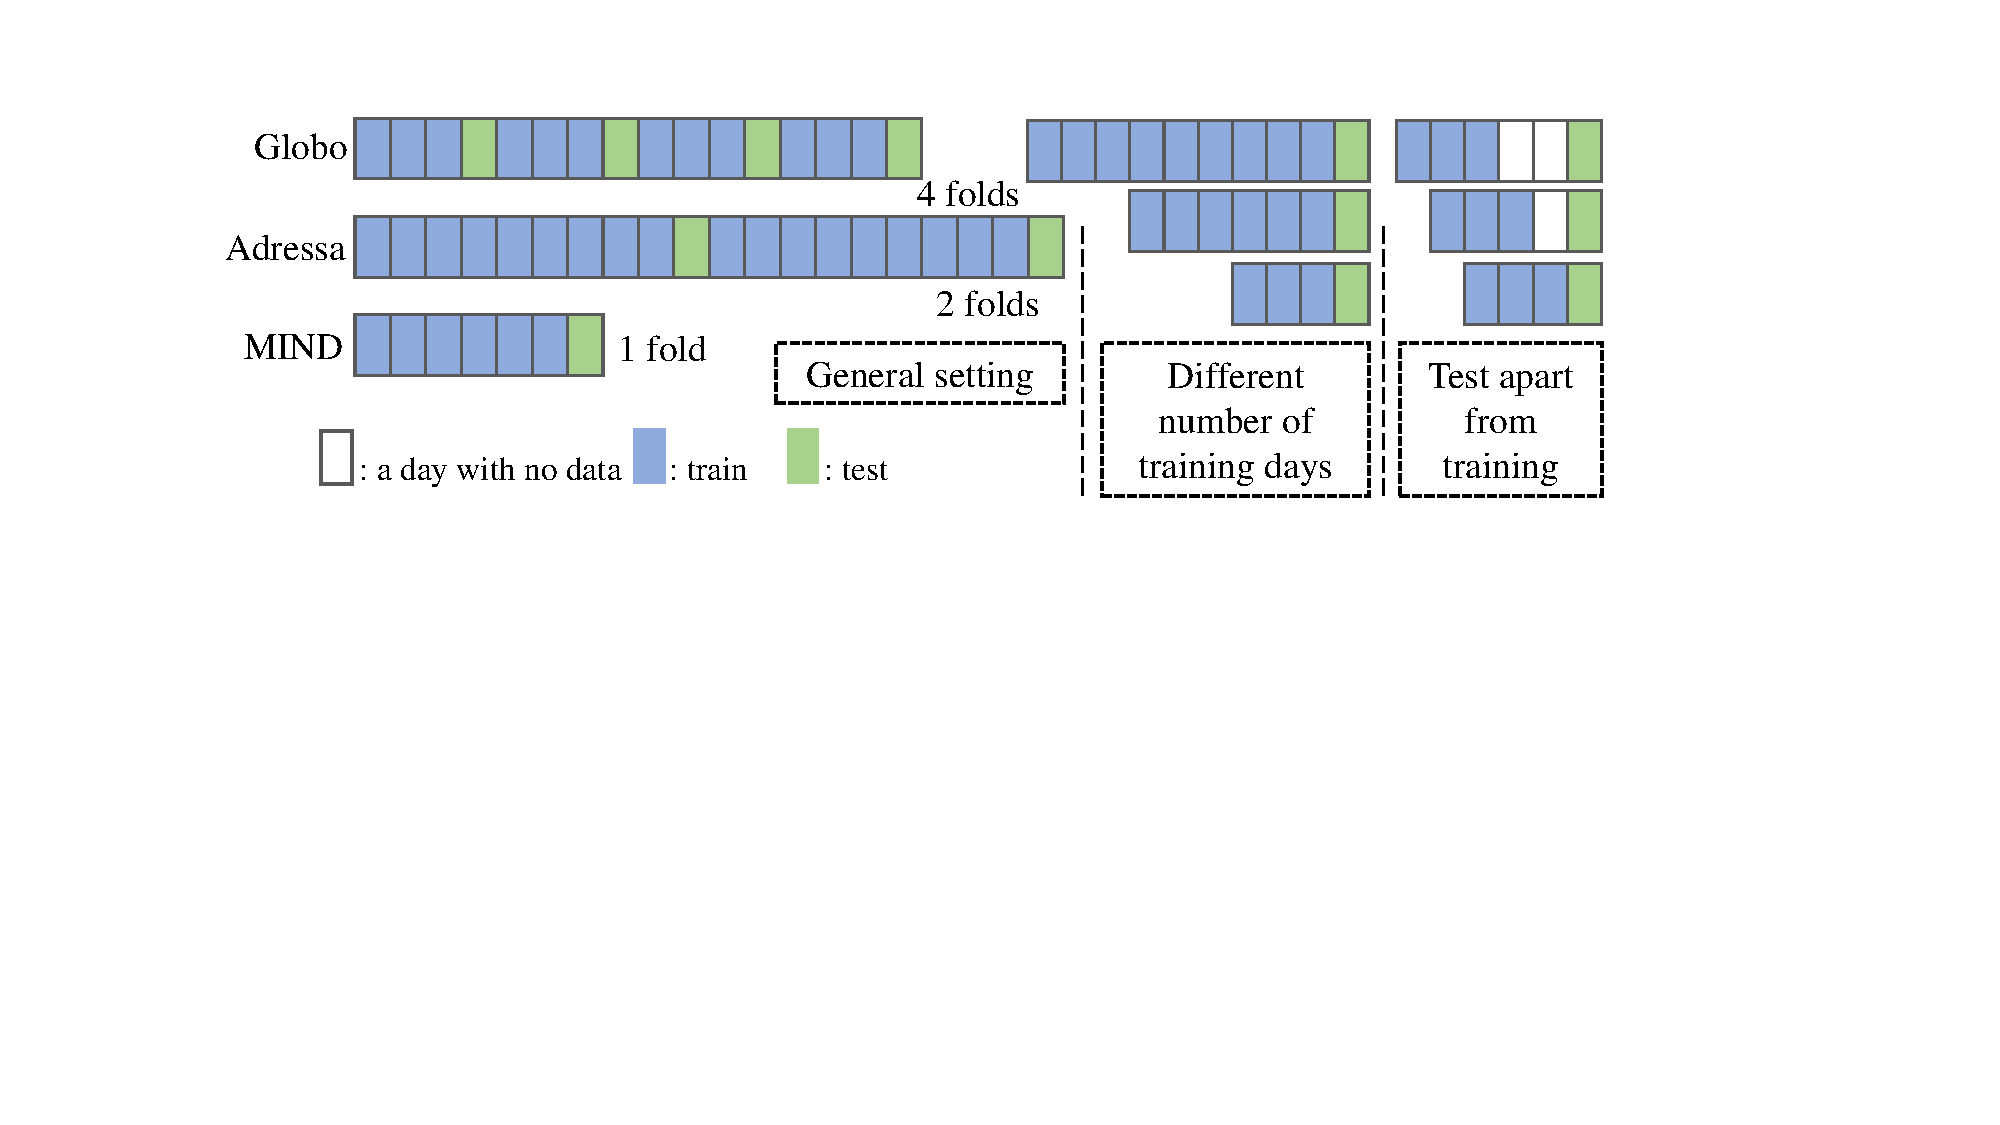
\includegraphics[width=\columnwidth]{fig/data_split.pdf}
%  \caption{Dataset splits to simulate different scenarios.}
%  \label{fig:data_split}
%  \Description[Data split]{An illustration of train/test set split.}
%\end{figure}

\subsubsection{Metrics}
During the test, given the first few click events in a session, the model generates 
a top-$k$ recommendation list $R$ with descending probabilities. 
We use widely-used metrics HR@$k$ (Hit Rate), NDCG@$k$ (Normalized Discounted Cumulative Gain) to 
measure the model's prediction accuracy.

Intra List Diversity (ILD@$k$)~\cite{symeonidis2020session} evaluates the topical/semantic 
diversity in $R$, and reflects the model's ability to recommend different items to the same user. 
\begin{equation}
  ILD@k = \frac{1}{|R|(|R|-1)}\sum_{a\in R}\sum_{b\in R}d(a,b),
\end{equation}
where $d(a, b)$ is a distance measure between item $a$ and $b$, and 
$d(a, b) = 1$ if item $a, b$ belong to different topics (categories), 0 otherwise.

Besides, we expect the system to recommend unseen items to surprise users. Content-based unexpectedness metrics (unEXP)~\cite{kaminskas2014measuring} can be used to measure this kind of unexpectedness, which is calculated as follows:

\begin{equation}
  unEXP_u@k = \frac{1}{|R|}\sum_{a\in R}\frac{1}{|S_u|}\sum_{b\in S_u}d(a,b).
\end{equation}

% According to~\cite{gabriel2019contextual}, we considered Item Coverage(COV@$k$) and novelty metrics ESIR@$k$ (Expected Self-Information with Rank-sensitivity) as additional metrics. COV@$k$ is also called ``aggregate diversity'', and reflects the model's ability to recommend different items
% to different users, which forces model to make a larger fraction of the item catalog visible to the users. We compute COV@$k$ as the number of distinct articles that appeared in any $R$ divided by the number of distinct last clicked articles in test set. ESIR@$k$ computes the novelty of item based on its popularity, returning higher values for long-tail items
% \begin{equation}
%   ESIR@k = \frac{\sum_{rank=1}^{k}-\log_2p(n_{rank})*disc(rank)}{\sum_{rank=1}^{k}disc(rank)},
% \end{equation}
% where $p(n_j)=\frac{recent\_clicks(n_j)}{\sum_{j \in N} recent\_clicks(n_j)}$ is the normalized popularity for long-tail items, and $disc(rank)=\frac{1}{\log_2(1+rank)}$ is a rank discount to emphasize a higher effect of items that is in the top positions of $R$.

\begin{table*}[th]\setlength{\tabcolsep}{7.5pt}
  \caption{Main results ($k=20$ by default in our all tables). All results are averaged over all folds. The best baseline result on 
  each metric is marked with $*$ and overall best results are bolded. The last column is our whole model.}
    \label{performance-table}
    \centering
    \renewcommand{\arraystretch}{1.3}
    \begin{tabular}{|c|c|ccccccccc|c|}
    \hline
    Datasets&Metrics&CB&CF&CBCF&STAN&GRU4Rec&SASRec&SRGNN&SGNNHN&STAMP&Ours \\ 
    \hline
    \multirow{5}{*}{Adressa} & HR & 0.0070 & 0.0924 & 0.0957 & 0.1130 & 0.1120 & 0.1205 & 0.1152 & 0.1285 & 0.1287$^*$ & \textbf{0.1658} \\ 
    \cline{2-12}
    & NDCG & 0.0024 & 0.0329 & 0.0341 & 0.0500 & 0.0511 & 0.0509 & 0.0536 & 0.0562 & 0.0575$^*$ & \textbf{0.0730} \\ 
    \cline{2-12}
    & ILD & 0.1131 & 0.8249 & 0.2337 & 0.2409 & 0.8170 & 0.7856 & \textbf{0.8611}$^*$ & 0.8403 & 0.8445 & 0.8085\\ 
    \cline{2-12}
    & unEXP & 0.1938 & 0.8243 & 0.2509 & 0.2407 & 0.6949 & 0.8010  & 0.4754
  & 0.8059$^*$ & 0.5728 & \textbf{0.8279} \\ 
    \cline{2-12}
    % & COV & 4.6208 & 2.4893 & 4.8021 & 1.2128 & 1.9794 & 1.3701 & 2.2872 & 0.0635 & 1.3429 & 1.6878 \\ 
    % \cline{2-12}
    % & ESIR & 17.98 & 18.13 & 17.87 & 5.058 & 9.507 & 16.60 & 7.863 & 9.074 & 16.64  & 8.835 \\ 
    % \cline{2-12}
    \hline
    % \cline{1-14}
    \multirow{5}{*}{Globo} & HR & 0.0355 & 0.1105 & 0.1185 & 0.1273 & 0.1280 & 0.1409 & 0.1280 & 0.1414 & 0.1435$^*$ & \textbf{0.1852}\\ 
    \cline{2-12}
    & NDCG & 0.0137 & 0.0437 & 0.0474 & 0.0647 & 0.0599 & 0.0620 & 0.0627 & 0.0611 & 0.0698$^*$ & \textbf{0.0936}\\ 
    \cline{2-12}
    & ILD & 0.2736 & 0.9253 & 0.3874 & 0.3087 & 0.9377 & \textbf{0.9864}$^*$ & 0.9248 & 0.9415 & 0.7980 & 0.8702\\
    \cline{2-12}
    & unEXP & 0.3112 & 0.9289 & 0.3730 & 0.2921 & \textbf{0.9771}$^*$ &0.9690   & 0.6383  & 0.9467 &  0.8437 & 0.8358 \\ 
    \cline{2-12}
    % & COV & 4.3960 & 1.7734 & 4.3734 & 0.9771 & 0.3492 & 0.8960 & 0.6782 & 0.0746 & 1.2494 & 1.3839 \\ 
    % \cline{2-12}
    % & ESIR & 18.232 & 18.256 & 18.188 & 5.8354 & 8.1474 & 16.26 & 7.0920 & 9.4295 & 15.534 & 10.134\\  
    \hline
    % \cline{1-14}
    \multirow{5}{*}{MIND} & HR & 0.0132 & 0.0248 & 0.0315 & 0.0312 & 0.0338 & 0.0355 & 0.0334 & 0.0366 & 0.0371$^*$ & \textbf{0.0495}\\ 
    \cline{2-12}
    & NDCG & 0.0047 & 0.0088 & 0.0110 & 0.0142 & 0.0132 & 0.0139 & 0.0144 & 0.0122 & 0.0151$^*$ & \textbf{0.0211}\\
    \cline{2-12} 
    & ILD & 0.0548 & 0.8268 & 0.7166 & 0.3193 & 0.8662 & 0.8562 & 0.8706 & 0.8775$^*$ & 0.8452 & \textbf{0.8813}\\ 
    \cline{2-12}
    & unEXP & 0.0972 & 0.8223 & 0.6039 & 0.1064 & 0.8578 & \textbf{0.8654}$^*$ & 0.4508 & 0.4514 & 0.7544 & 0.8617 \\ 
    \cline{2-12}
    % & COV & & &   &   &   &   &   &  &   &  \\ 
    % \cline{2-12}
    % & ESIR & & &  &   &   &   &   &   &   &  \\ 
    % \cline{2-12}
    \hline
  \end{tabular}
  \end{table*}


\subsubsection{Baseline Algorithms}
These are the strong baselines for comparison. Despite the simplicity of some of those methods, they still have competitive accuracy on session-based recommendations.

\noindent
\textit{Simple approaches without deep learning:}

\textit{CBCF}~\cite{sottocornola2018session} is a news recommender combines Content-Based similarity with session-based Collaborative Filtering similarity.

\textit{STAN}~\cite{garg2019sequence} is an extended version of SKNN (Session-KNN) with three controllable temporal decay factors. In experiments, we choose the best weighting factors for CB similarity and CF similarity in the experiment. We also list the results of separate CB and CF as a reference.

\noindent
\textit{Session-based neural recommenders:}

  \textit{GRU4Rec}~\cite{hidasi2015session,hidasi2018recurrent} is a Gated Recurrent Unit for recommendation, building with gated recurrent neural networks, which is similar to LSTM in ~\cite{gabriel2019contextual}.

  \textit{SASRec}~\cite{kang_self-attentive_2018} is a self-attention based Sequential model, adopting Transformer architecture to model user's action.
  
  \textit{STAMP}~\cite{liu2018stamp} is a Short-Term Attention/Memory Priority Model for Session-based Recommendation, introducing the attention mechanism to model the relationship of each historical click and the last click.

  \textit{SRGNN}~\cite{wu2019session} is a Session-based Recommender using Graph Neural Networks to capture complex transitions of items.

  \textit{SGNNHN}~\cite{pan2020star} is improved SR-GNN using Star Graph Neural Network.

  For session-based neural recommenders, we initialize the item embeddings with items' content vector for fair comparation.

\noindent
\textit{Neural news recommendation approaches:}

\textit{CPRS}~\cite{wu2020CPRS} is a typical news recommendation approach that utilizes the textual feature of articles to model user's interests. It also uses the dwell time (i.e. active time) to measure user's satisfaction. We make this approach adapt to the session-based scenario. Since only Adressa dataset contains complete information for CPRS, we only compare it with our method in Adressa dataset which is discussed in \tabref{tb:CPRS}.

\subsubsection{Implementation Details}
For fair comparisons, we apply all baselines to the same augmented data and train 
models on one GTX1080Ti GPU.
We use the same latent dimensions $d_n=d_c=250, d_t=64$, choose different learning rate $\{0.002, 0.001, 0.0005\}$, batch size $\{512, 1024, 2048\}$ and other hyper-parameters to select the best model using early stopping strategy based on the HR@20 score on the validation set, which is the last 10\% of samples in the training set sorted by time. All embedding tables are normally initialized with 0 mean, 0.002 standard deviation, and for weighting parameters 0 mean, 0.05 standard deviation.

\subsection{Main Results}
\label{sec:mainres}

In \tabref{performance-table} and \figref{fig:all}, we compare the performance of all baselines and our
approach, and we can make the following observations.

Non-neural methods CBCF and STAN are either considering the content 
information or the recency of the current session, and their results are somehow 
comparable to deep learning methods in three datasets. However, they generate recommendation lists with low diversity/novelty, mainly because their simple algorithms cannot capture enough personalized information. For session-based approaches, generally speaking, STAMP and SGNNHN yield better performance on HR and NDCG, but not always good at ILD/unEXP, while SASRec and SRGNN recommend more diverse but less accurate, showing the trade-off between diversity and accuracy. From the user's aspect, though, when ILD/unEXP is over a threshold (like 0.80), it's hard for them to distinguish the difference, thus the ILD/unEXP score of our model is bearable. 

As for our whole model, when compared with STAMP, it performs better or close on both accuracy and diversity. This result shows that \textbf{our model mitigates the dilemma between accuracy and diversity} 
to a certain extent. In the MIND dataset, 
the improvement is comparatively small and the possible reasons are: 
on the one hand, MIND did not provide active interval, nor did they give click time of each article (just start time of a session), 
we cannot get positive feedback from the data; on the other hand, from the results of CBCF, 
we assume the article transition information is too sparse and thus it is hard to recommend. 
Note that this dataset is not designed for the session-based recommendation, hence some information 
may be inaccurate (e.g., one session may last for days, longer than 30 minutes).

\begin{figure*}[th]
\begin{subfigure}[b]{0.48\textwidth}
\centering
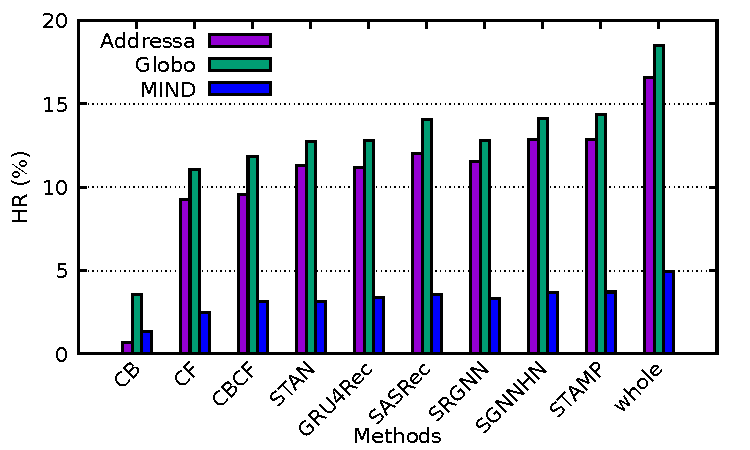
\includegraphics[width=\columnwidth]{fig/hr.pdf}
\caption{HR}
\label{fig:hr}
\end{subfigure}
\hfill
\begin{subfigure}[b]{0.48\textwidth}
\centering
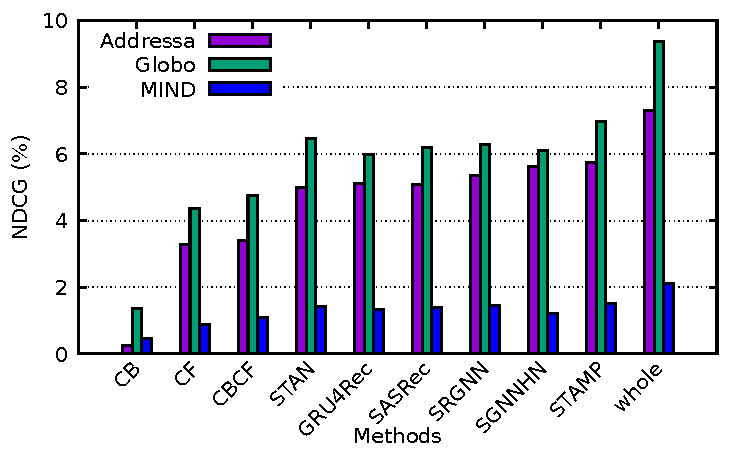
\includegraphics[width=\columnwidth]{fig/ndcg.pdf}
\caption{NDCG}
\label{fig:ndcg}
\end{subfigure}
\begin{subfigure}[b]{0.48\textwidth}
\centering
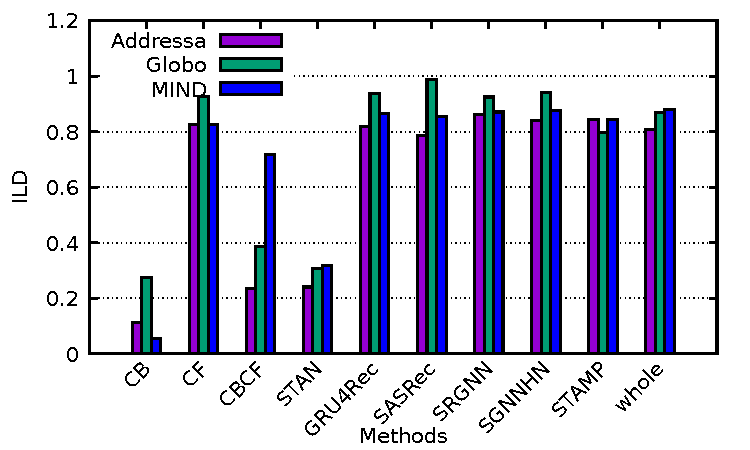
\includegraphics[width=\columnwidth]{fig/ild.pdf}
\caption{ILD}
\label{fig:ild}
\end{subfigure}
\hfill
\begin{subfigure}[b]{0.48\textwidth}
\centering
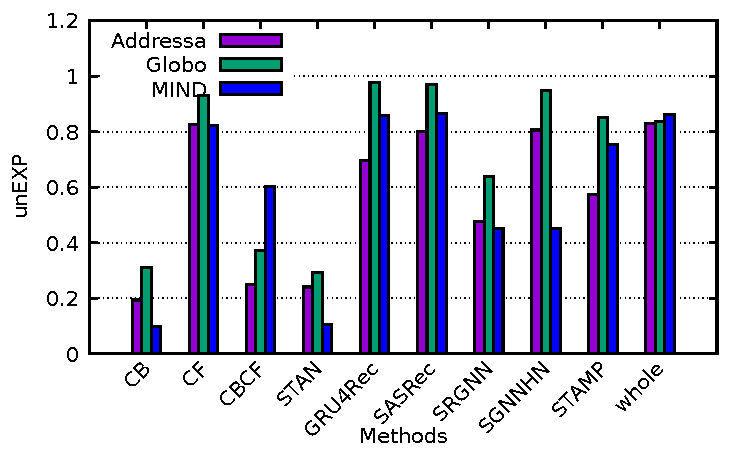
\includegraphics[width=\columnwidth]{fig/unexp.pdf}
\caption{unEXP}
\label{fig:unexp}
\end{subfigure}
\caption{The graphical comparison of all methods on 4 different metrics and 3 different datasets.``Whole'' is our approach.}
\label{fig:all}
\end{figure*}

\subsection{Effectiveness of Components}
\begin{table}[th]\setlength{\tabcolsep}{3.5pt}
  \caption{The ``whole'' is our whole model, and (-) means to ablate the corresponding module. The last column is to replace our negative sampling strategy with random sampling. 
  $\downarrow$ indicates performance drop over the whole model.}
    \label{ablation}
   \renewcommand{\arraystretch}{1.3}
    \centering
    \begin{tabular}{|c|c|ccccc|}
    \hline
    Datasets&Metrics&whole&(-)neutral&(-)pos&(-)neg& with random\\ 
    \hline
    \multirow{3}{*}{Adressa} & HR & 0.1658 & 0.1344$\downarrow$ & 0.1619$\downarrow$ & 0.1658 &0.1646$\downarrow$\\ 
    \cline{2-7}
    & NDCG & 0.0730 & 0.0613$\downarrow$ & 0.0690$\downarrow$ & 0.0720$\downarrow$ &0.0693$\downarrow$\\ 
    \cline{2-7}
    & ILD & 0.8085 & 0.8204 & 0.8249 & 0.8237 &0.8234\\ 
    \cline{2-7}
    & unEXP & 0.8279 & 0.8243$\downarrow$ & 0.8333 & 0.8267$\downarrow$ &0.8346\\ 
    \hline
    % \cline{1-14}
    \multirow{3}{*}{Globo} & HR & 0.1852 & 0.1460$\downarrow$ & 0.1817$\downarrow$ & 0.1821$\downarrow$ &0.1847$\downarrow$\\ 
    \cline{2-7}
    & NDCG & 0.0936 & 0.0727$\downarrow$ & 0.0907$\downarrow$ & 0.0940 &0.0933$\downarrow$\\ 
    \cline{2-7}
    & ILD & 0.8702 & 0.8362$\downarrow$ & 0.8685$\downarrow$ & 0.8927 &0.8739\\ 
    \cline{2-7}
    & unEXP & 0.8358 & 0.8142$\downarrow$ & 0.8252$\downarrow$ & 0.8489& 0.8317$\downarrow$\\ 
    \hline
    % \cline{1-14}
    \multirow{3}{*}{MIND} & HR & 0.0495 & 0.0445$\downarrow$ & - & 0.0471$\downarrow$ &0.0457$\downarrow$\\ 
    \cline{2-7}
    & NDCG & 0.0211 & 0.0198$\downarrow$ & - & 0.0180$\downarrow$ &0.0204$\downarrow$\\
    \cline{2-7} 
    & ILD & 0.8813 & 0.8779$\downarrow$ & - & 0.8808$\downarrow$ &0.8858\\
    \cline{2-7}
    & unEXP & 0.8617 & 0.8415$\downarrow$ & - & 0.8623&0.8680\\  
    \hline
  \end{tabular}
  \end{table}
% \label{sec:abla}
From \tabref{ablation} we can verify the effects of modeling user positive negative and neural implicit feedback in our model. Compared with the whole model, there is a huge drop after removing neural information and this is the most consistent over all metrics, which reveals the importance of neural information (temporal information), and we will discuss the modeling of it in detail (\secref{sec:t}). Adressa 
 provides \textbf{the most complete information}, which not only releases the original 
text of articles instead of the extracted vectors in Globo, but also gives the accurate active time 
of the user in each article, while we can only estimate the active time by the interval between 
two successive clicks for Globo, which may not be accurate. However, the positive information performs similarly in both Adressa and Globo dataset, implying that our approximate estimation is reasonable. We observe that negative information is less effective than positive information, especially by diversity/novelty metrics. 
One explanation is that the negative samples from the impression list are reconstructed based on their publishing time, so the information is not totally reliable. Negative sampling module lowers diversity, possibly because in the dataset the negative samples and the positive article usually belong to different categories, thus adding this module forces the model to recommend similar articles to the positive one. Negative feedback is better modeled in MIND due to its complete impression data. To verify the effect of the negative sampling strategy more accurately, we set the control group with random sampling, and we find that even though the random sampling would decrease the performance slightly, our negative feedback shows superior performance over it. The possible reason for the worse performance of using random sampling is that randomly sampled negative items have the possibility to be liked by this user, and this module imports some noise instead because this sample strategy does not consider \textbf{what the user really likes}. 
We cannot get positive feedback from MIND so this column is empty, and the reasons why the improvement is limited for MIND are analyzed previously.

\subsection{Effects of Positive Feedback}
CPRS considers the active time to represent the user's satisfaction using personalized reading speed, which is quite similar but more complex than our positive feedback modeling. We first modify this method to meet the 
session-based scenario, and second plug the personalized reading speed into our model. 
The experiment is conducted in Adressa due to its complete information 
(Globo does not provide the text-level content and the active time is missing for MIND). 
In \tabref{tb:CPRS}, the poor score of CPRS shows that when it is adapted to the session-based scenario, 
limited interactions are the bottleneck. When we adopt their personalized reading speed instead of 
the reading time, there is no significant improvement, and we hypothesize that for this dataset, 
when news reading \textbf{the reading speed is quite similar} for different users.

\begin{table}[th]\setlength{\tabcolsep}{8pt}
  \caption{Results of CPRS and CPRS module plugged into our model in Adressa dataset.}
  \label{tb:CPRS}
  \centering
  \renewcommand{\arraystretch}{1.3}
  \begin{tabular}{|c|cccc|}
    \hline
    % \multicolumn{2}{c}{Part}                   \\
    % \cmidrule(r){1-2}
    Methods  & HR & NDCG & ILD & unEXP\\
    \hline
    Our whole model & 0.1658 & 0.0730 & 0.8085 & 0.8279\\
    \hline
    CPRS & 0.0812 & 0.0371 & 0.8191 & 0.8109\\
    Ours using speed & 0.1641 & 0.0674 & 0.8457 & 0.8245\\
    Ours using 1-d $t_i$ & 0.1603 & 0.0705 & 0.8293 & 0.8220\\
    \hline
  \end{tabular}
\end{table}

To verify the effectiveness of the duration encoder, we compare it with the continuous active time vector $t_i$ regarded as a one-dimensional vector instead of using distinct categories. As the result shows, the accuracy score of 1-d $t_i$ is inferior to our whole model, indicating that our duration encoder catch more personalized information by bucketizing it.

\subsection{Effects of Negative Feedback}
In this section, we first validate our assumption for the negative user feedback,
which is that articles whose publishing time is close to the clicked articles are
likely presented to the user, or within their impressions.
We do that on the MIND dataset, in which the real impressions and the
publishing time of articles are all available for the sessions. 
For each session $S_u$, we sample negative items $Ne_u$ using our strategy, and compute Jaccard similarity between $Ne_u$ and real $Imp_u$, the overall score is 0.0062 when $|Ne_u=100|$, compared with 0.0044 when random sampling.
This shows that our assumption is reasonable and our strategy can \textbf{better reconstruct the impression list}.

We further conduct a parameter analysis on loss weights $\lambda$ and the number of negative samples $|Ne|$ 
in \eqnref{eq:loss}. We report results on Adressa as an example, and results from other datasets are similar. 
The number of negative samples does not matter much, as shown in \figref{fig:para_a}, 
so for simplicity we choose $|Ne|=20$. The performance gets worse if $\lambda$ is set too low or too 
high in \figref{fig:para_b}, we conclude that the negative loss is useful but too many weights on it will \textbf{harm} the learning of the user's positive feedback.

\begin{figure}[th]
  \centering
  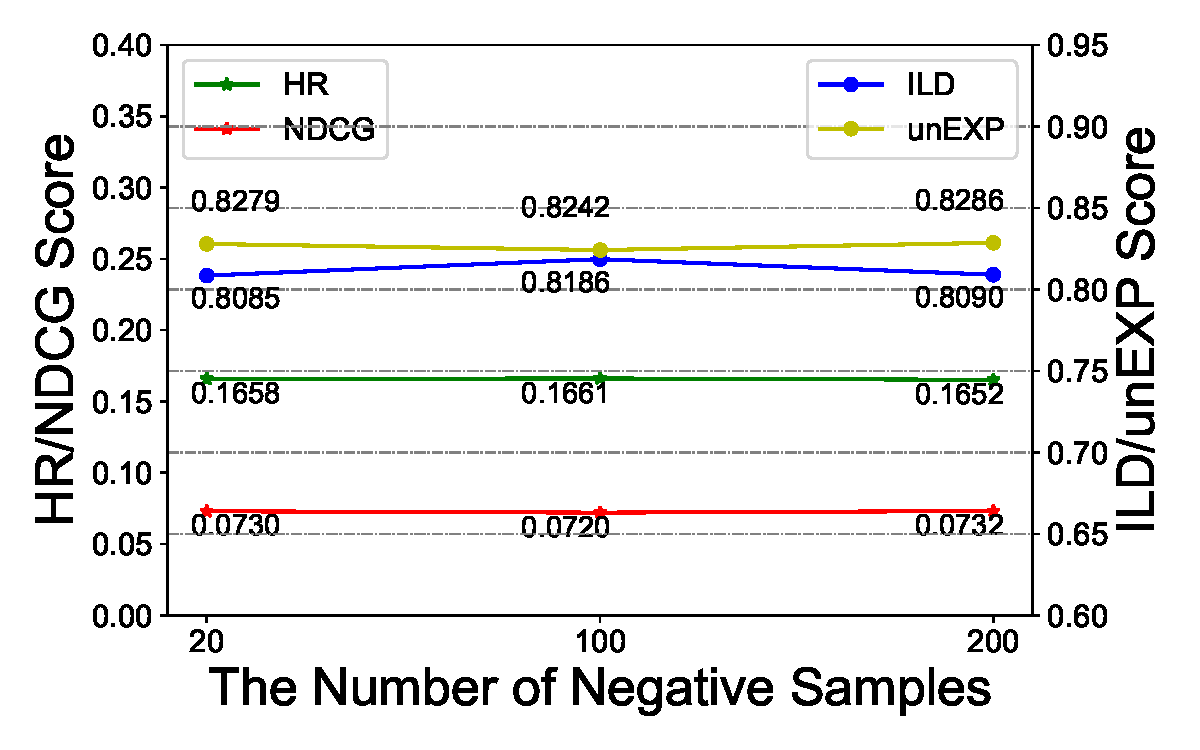
\includegraphics[width=0.8\linewidth]{fig/parameter_a.pdf}  
  \caption{Results for different $|Ne|$.}
\label{fig:para_a}
\end{figure}

\begin{figure}[th]
  \centering
  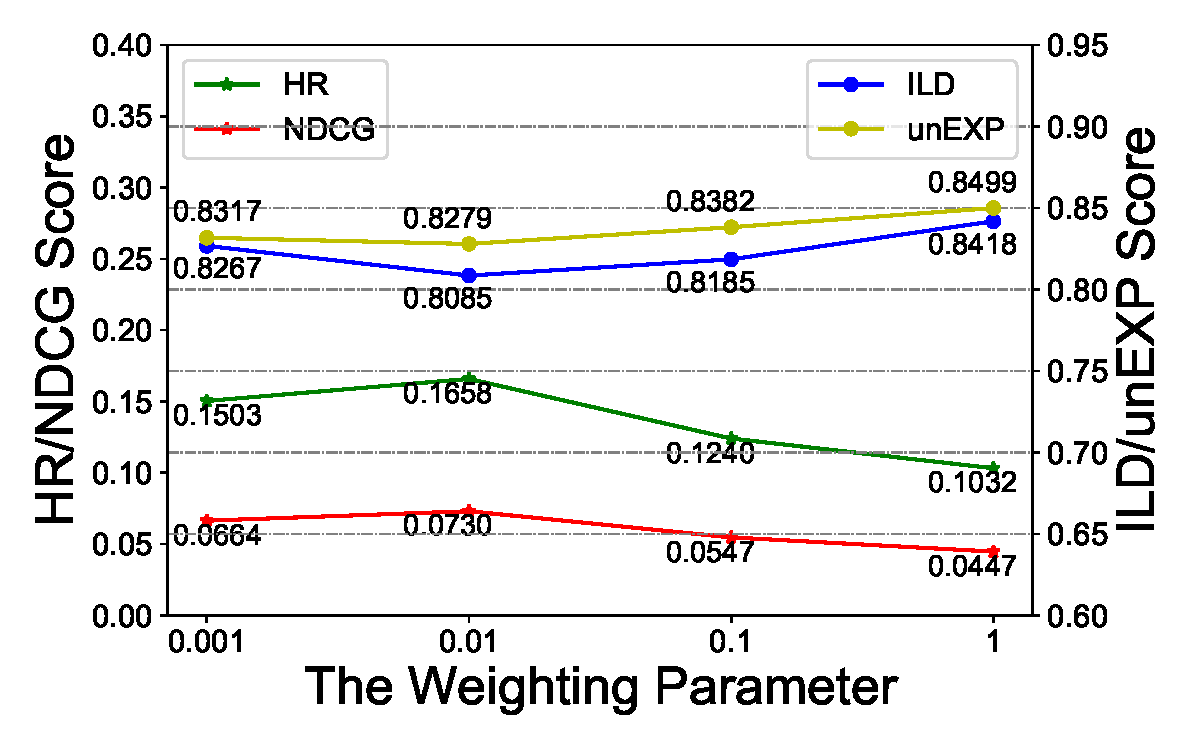
\includegraphics[width=0.8\linewidth]{fig/parameter_b.pdf}  
  \caption{Results for different $\lambda$.}
  \label{fig:para_b}
\end{figure}

\subsection{Temporal Representations}
\label{sec:t}
Since both the start time and the publishing time use the temporal encoder, 
we wonder if it would be better to have them share the embedding space. 
\tabref{tb:temporal} shows the findings. 

\begin{table}[th]
  \caption{Different ways of utilizing temporal information, where ``p'' stands for the publishing time and ``s'' stands for the start time. }
  \label{tb:temporal}
  \centering
  \renewcommand{\arraystretch}{1.3}
  \begin{tabular}{|c|cccc|}
    \hline
    % \multicolumn{2}{c}{Part}                   \\
    % \cmidrule(r){1-2}
    Methods  & HR & NDCG & ILD & unEXP \\
    \hline
    whole (shared) & 0.1658 & 0.0730 & 0.8085 & 0.8279\\
    whole (no share) & 0.1620 & 0.0727 & 0.8310 & 0.8215\\
    \hline
    whole-p-s & 0.1353 & 0.0612 & 0.8280 & 0.8276\\
    whole-p & 0.1344 & 0.0613 & 0.8204 & 0.8243\\
    whole-s & 0.1620 & 0.0726 & 0.8325 & 0.8415\\
    \hline
  \end{tabular}
\end{table}

We can see that sharing the time embedding between publishing time and
session start time has clear advantages in most of the metrics. This is
because publishing time is associated with every article and there are a lot of
such data for training, whereas the session start time suffers from lack
of data and is less trained. Training the two jointly implicitly helps each 
other. It also makes physical sense because a Monday is a Monday regardless
a story breaks on that day or a reader pops in to read that story on that day.

The ablation tests of using only publishing time or only start time in
\tabref{tb:temporal} also clearly indicates that temporal modeling both from
the item point of view and the user point of view are useful in garner latent
information between the two. In other words, \tabref{tb:temporal} shows that
the neutral feedback works.

To give some concrete evidence that the time embedding that we train
carries some physical meanings, we visualize the embedding tables for
\textit{minutes}, \textit{hours}, \textit{weekdays} and \textit{days
of a month}, in \figref{fig:temporal}, which is trained on a subset of the Adressa dataset.
Some interesting patterns can be observed. For example, the representation
of the minutes are rather uniform and random, because news publishing and
reading can happen any minute of an hour. But there are certainly more
activities at certain hours during a day (such as 10 am). There are also
some irregular patterns for Monday and Sunday as shown in (c).
Finally, because we only have the first 15 days of training data in this dataset,
values for dates 16-31 in (d) are not fully trained, which only has the chance to update when the publishing date of articles falls in the range of 16-31, but most of articles are published nearby the click time according to the dataset statistics.
\begin{figure*}[th]
  \centering
  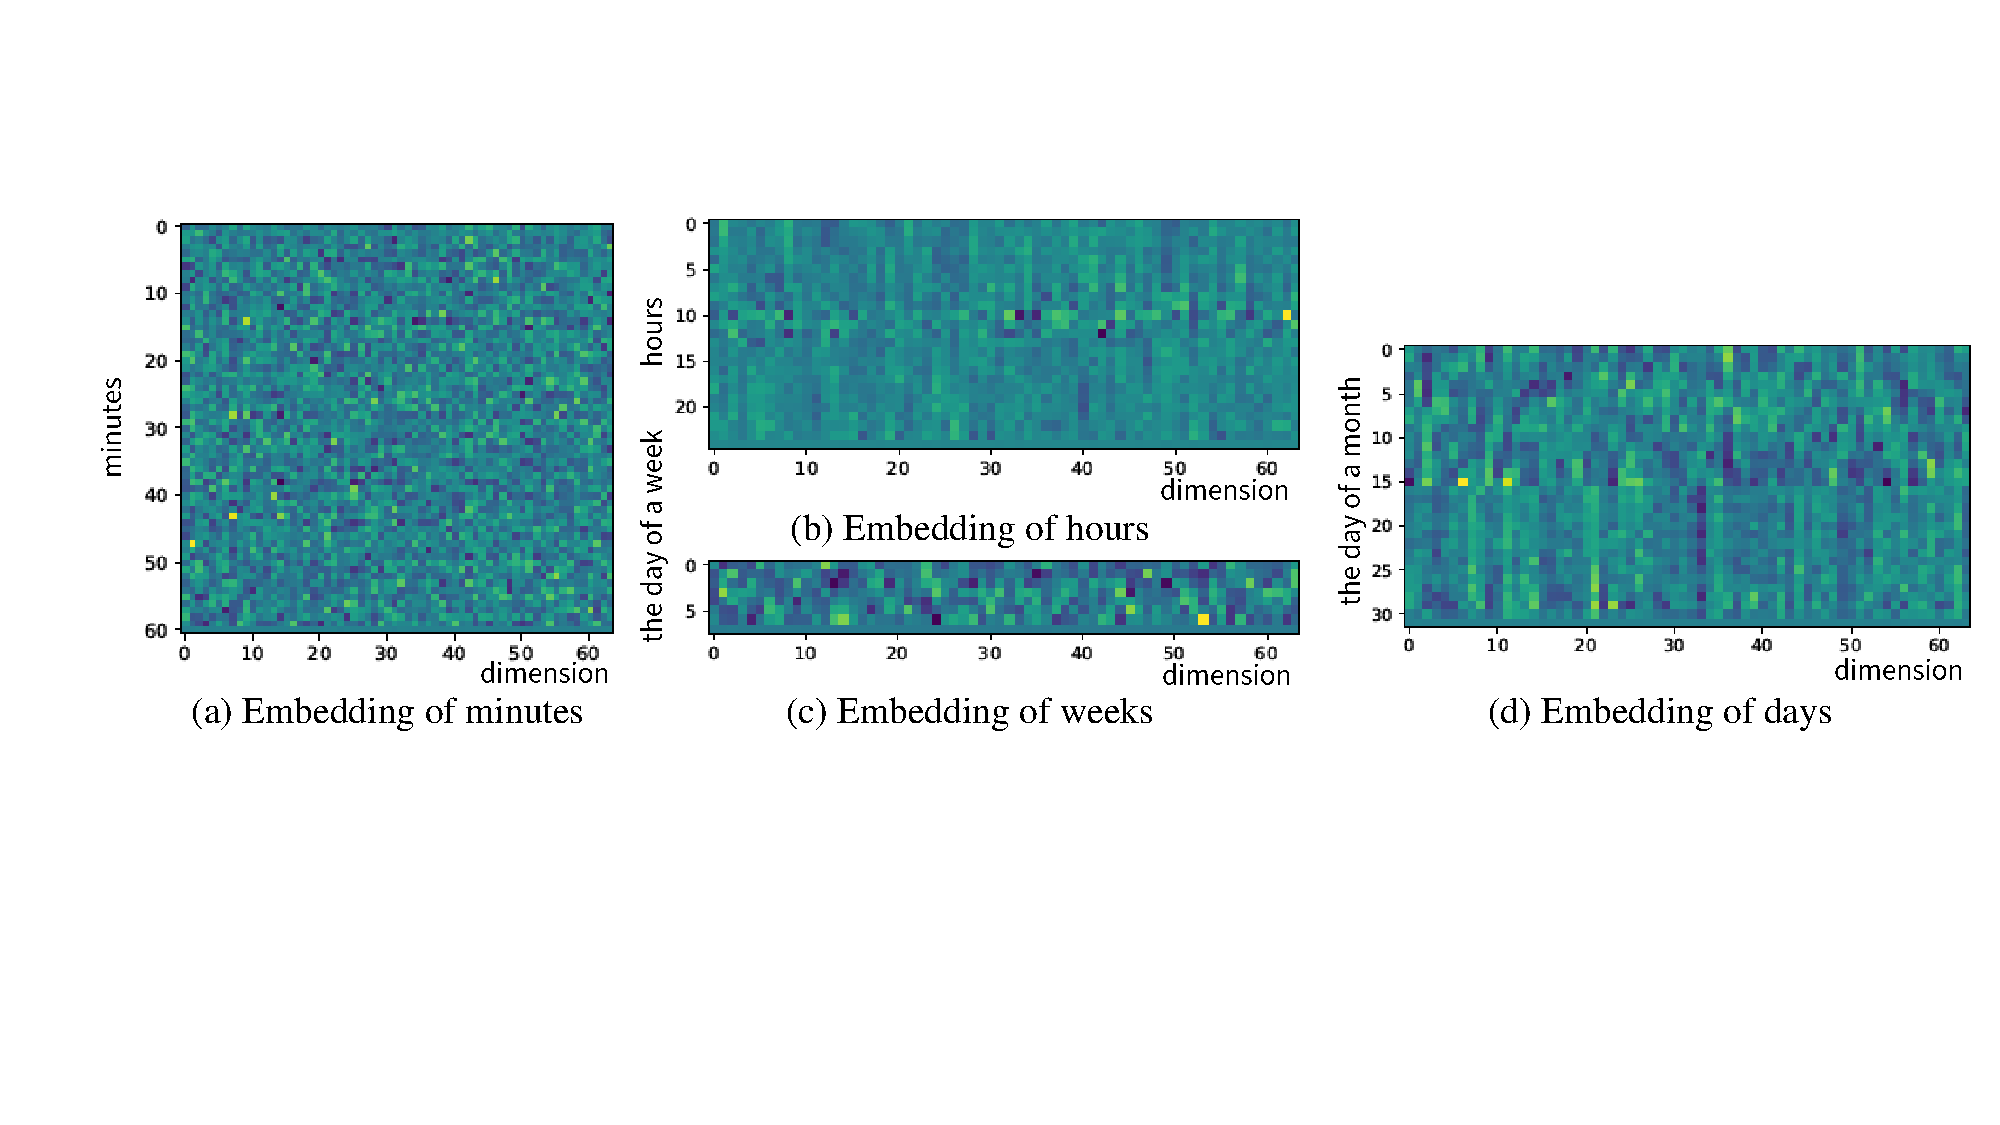
\includegraphics[width=0.9\textwidth]{fig/visualization.pdf}  
  \caption{The visualization of time embedding tables for the day of a month, the day of a week, hour and minute, trained on Addressa dataset.}
  \label{fig:temporal}
\end{figure*}


\subsection{Discussion}
\label{sec:discuss}

\subsubsection{Article cold-start}
\label{sec:itemcold}
For news recommendation, all methods suffer from article cold-start problem due to the continuously published news, the analyses of the article cold-start scenario can help us 
figure out where our improvement comes from. Another concern about the article cold-start problem is that if fresh articles can not get exposure reasonably, they will suffer from the Matthew effect and will not be clicked anymore. According to~\cite{gabriel2019contextual}, instead of using user-oriented metric ILD/unEXP, we thus consider the system-oriented Item Coverage(COV@$k$) as an additional metric. COV@$k$ is also called ``aggregate diversity'', and reflects the model's ability to recommend different items to different users, which forces the model to make a larger fraction of the item catalog visible to the users. We compute COV@$k$ as the number of distinct articles that appeared in any $R$ divided by the number of distinct last clicked articles in the test set. 
%In the article cold-start situation, none of the articles in input sequence is 
%observed during training, we need to recommend articles based on their content and from the user's implicit feedback. 
\tabref{tb:cold-start} lists the results of one fold in Globo dataset, and we choose it because it suffers from the most severe cold-start problem. 
For cold situation, where the test articles are completely disjoint from
the training data, STAN does badly because it can't handle unseen items.
Deep learning methods tend to predict the same articles for different users. 
Even though methods like SASRec yields not bad results, 
the models tend to overfit to popular articles. Our model, on the other hand, not only performs well on HR@20 but also gets the comparable COV@20 score, and the difference with the
other deep learning methods is remarkable. 
In non-cold situation, the performance of all methods is close. 
The overall recommendation results largely depend on how a method does for 
cold-start scenarios.

\begin{table}[!htp]
\caption{Cold start performance on Globo dataset in the first fold.}
\label{tb:cold-start}
\centering
\renewcommand{\arraystretch}{1.3}
\begin{tabular}{|c|c|c|c|c|c|c|}
  \hline
  \multirow{2}{*}{Methods}  & \multicolumn{2}{c|}{Cold(80.3\%)} & \multicolumn{2}{c|}{non-Cold(19.7\%)} & \multicolumn{2}{c|}{Total} \\ \cline{2-7} 
    & HR & COV & HR & COV & HR & COV   \\ 
  \hline
  CBCF & 0.0369   & 5.06  &  0.2488 & 5.54 & 0.0787  & 3.95 \\
  STAN & -  & - &  0.2652  &  1.63 & 0.0522   & 0.93  \\ 
  \hline
  GRU4Rec & 0.0151  & 0.03  & 0.2093 & 0.88 &  0.0533  & 0.50 \\
  SASRec & 0.0080  & 0.01  & 0.2335 & 1.28 & 0.0525 & 0.73 \\
  SR-GNN & 0.0100  & 0.01  & 0.2365 & 0.99  & 0.0546 & 0.57\\ 
  STAMP & 0.0172 & 0.01 & 0.2184  & 1.04 & 0.0568 & 0.59 \\
  SGNNHN & 0.0089 & 0.01 & 0.2486 & 0.05 & 0.0561 & 0.04 \\
  \hline
  Ours & 0.0496 & 0.74 & 0.2527  & 1.87  & 0.0896  & 1.20  \\
  \hline
\end{tabular}
\end{table}

\subsubsection{User cold-start}
\label{sec:usercold}
Since anonymous news sessions are short with the average length of less than 3, 
the user cold-start problem is severe. We show the results for different input lengths in 
\figref{fig:inputlen}. We report results on Globo, and other datasets perform similarly. Interestingly, our model reaches its peak accuracy from length 1 to 2. 
In contrast, other methods all reach the peak at 3.
This shows our model is capable of \textbf{capturing user interests earlier} in the session 
by leveraging the user's implicit feedback. For longer input length, 
the difference between our model and others narrows, 
indicating the similar ability to predict given longer history. We can observe that the performance drops with the longer length input, and this may contribute to the noise that is imported from the longer reading history, which means it is harder to recommend when considering the longer and more diverse interests from users.

\begin{figure}[th]
  \centering
  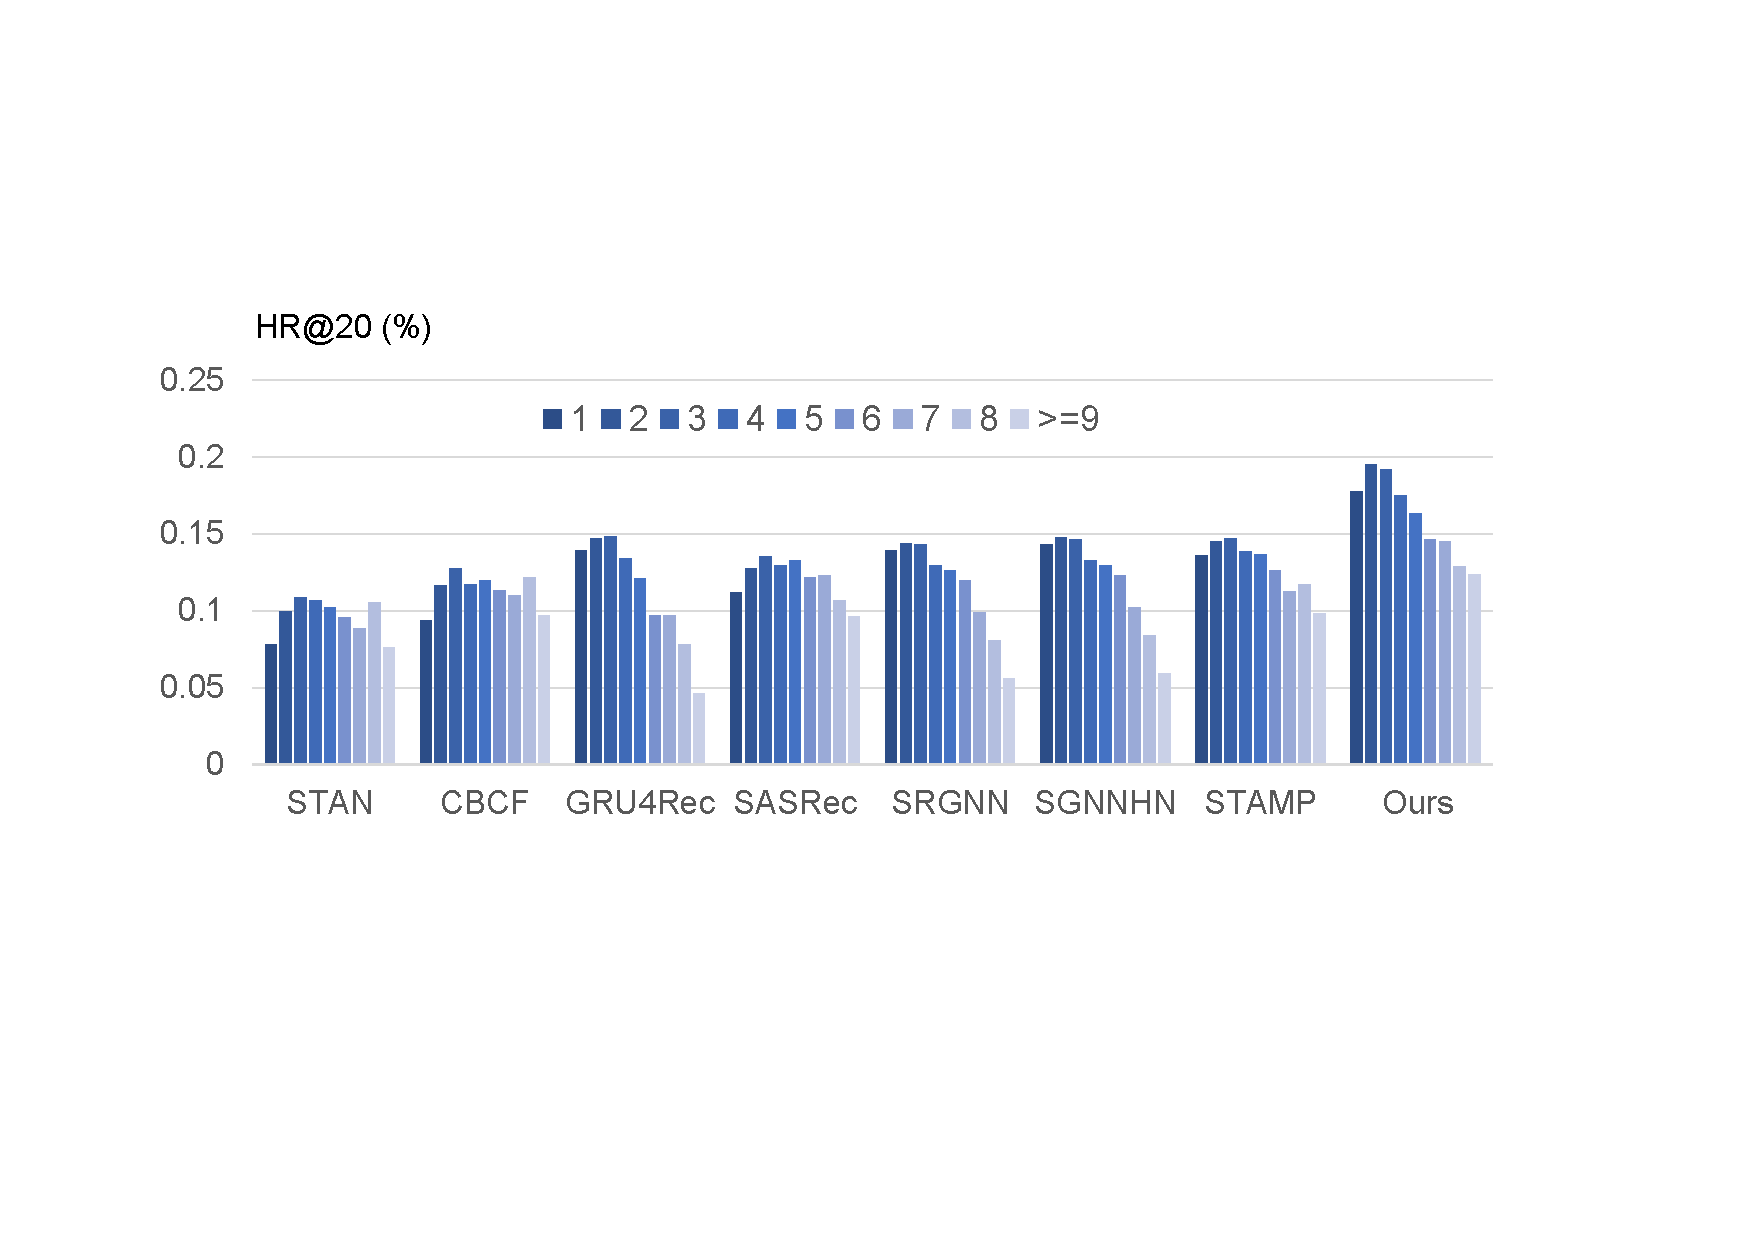
\includegraphics[width=0.95\columnwidth]{fig/input_len.pdf}
  \caption{Accuracy with different session lengths.}
  \label{fig:inputlen}
\end{figure}

\subsubsection{Different number of days for training}
\label{sec:robo}
We fix the 10th day in Globo dataset as the test data, and choose the different number of prior days to train. The result is shown in \figref{fig:trainlen}. The overall performance of our model is consistently 
better with large margins than all other methods and is stable regardless of the number of training days. 
Most other methods heavily rely on the freshness of items and they generally 
do better with closer training data. 

\begin{figure}[th]
  \centering
  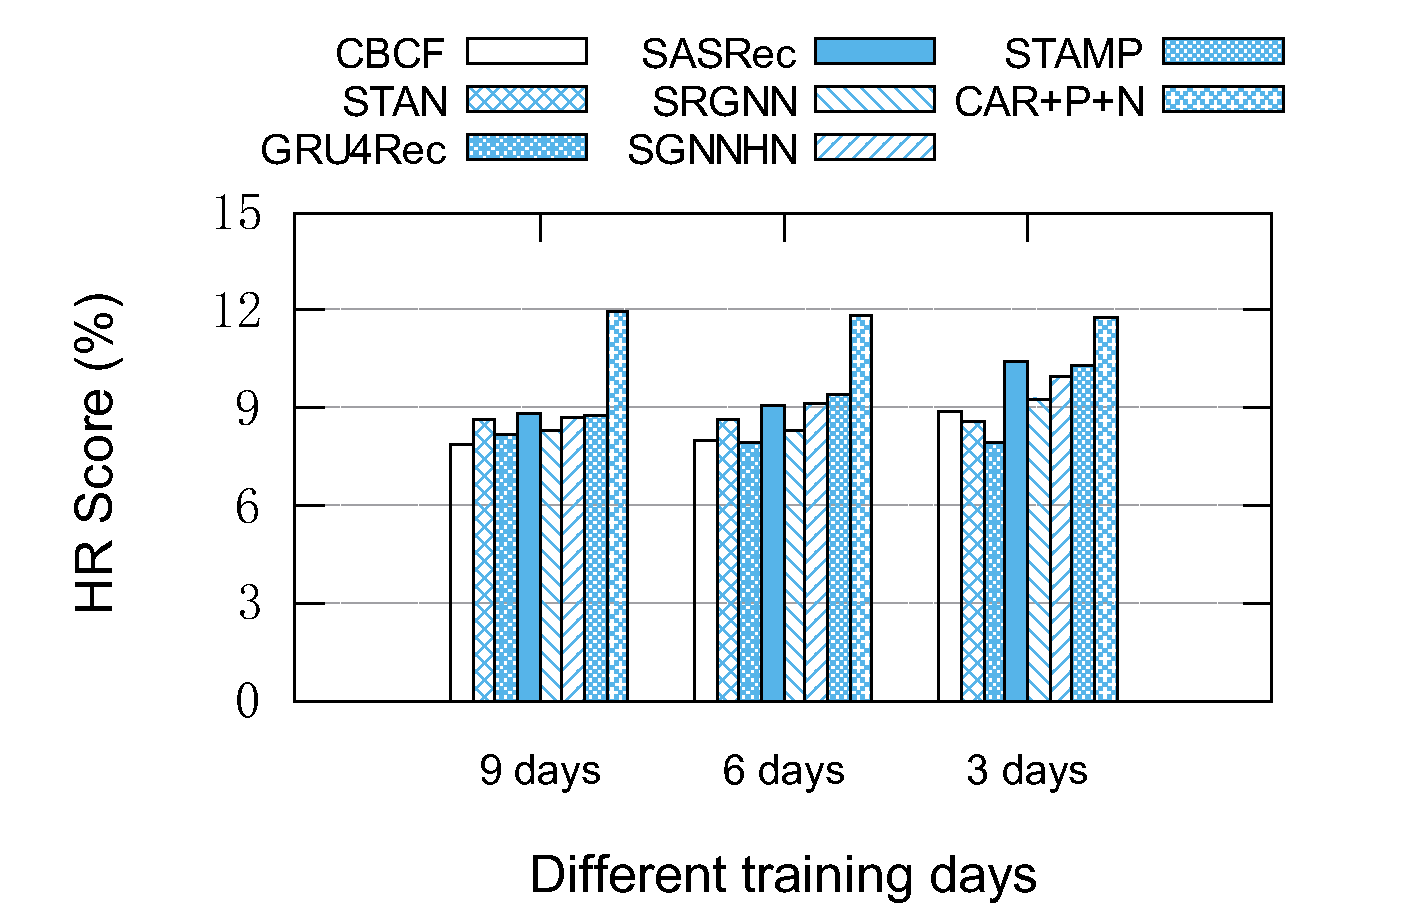
\includegraphics[width=0.8\columnwidth]{fig/diff_day_len.pdf}
  \caption{Accuracy under different training splits.}
  \label{fig:trainlen}
\end{figure}


